% Options for packages loaded elsewhere
\PassOptionsToPackage{unicode}{hyperref}
\PassOptionsToPackage{hyphens}{url}
%
\documentclass[
]{article}
\usepackage{amsmath,amssymb}
\usepackage{lmodern}
\usepackage{ifxetex,ifluatex}
\ifnum 0\ifxetex 1\fi\ifluatex 1\fi=0 % if pdftex
  \usepackage[T1]{fontenc}
  \usepackage[utf8]{inputenc}
  \usepackage{textcomp} % provide euro and other symbols
\else % if luatex or xetex
  \usepackage{unicode-math}
  \defaultfontfeatures{Scale=MatchLowercase}
  \defaultfontfeatures[\rmfamily]{Ligatures=TeX,Scale=1}
\fi
% Use upquote if available, for straight quotes in verbatim environments
\IfFileExists{upquote.sty}{\usepackage{upquote}}{}
\IfFileExists{microtype.sty}{% use microtype if available
  \usepackage[]{microtype}
  \UseMicrotypeSet[protrusion]{basicmath} % disable protrusion for tt fonts
}{}
\makeatletter
\@ifundefined{KOMAClassName}{% if non-KOMA class
  \IfFileExists{parskip.sty}{%
    \usepackage{parskip}
  }{% else
    \setlength{\parindent}{0pt}
    \setlength{\parskip}{6pt plus 2pt minus 1pt}}
}{% if KOMA class
  \KOMAoptions{parskip=half}}
\makeatother
\usepackage{xcolor}
\IfFileExists{xurl.sty}{\usepackage{xurl}}{} % add URL line breaks if available
\IfFileExists{bookmark.sty}{\usepackage{bookmark}}{\usepackage{hyperref}}
\hypersetup{
  pdftitle={Random variables: theory and practice},
  hidelinks,
  pdfcreator={LaTeX via pandoc}}
\urlstyle{same} % disable monospaced font for URLs
\usepackage[margin=1in]{geometry}
\usepackage{color}
\usepackage{fancyvrb}
\newcommand{\VerbBar}{|}
\newcommand{\VERB}{\Verb[commandchars=\\\{\}]}
\DefineVerbatimEnvironment{Highlighting}{Verbatim}{commandchars=\\\{\}}
% Add ',fontsize=\small' for more characters per line
\usepackage{framed}
\definecolor{shadecolor}{RGB}{248,248,248}
\newenvironment{Shaded}{\begin{snugshade}}{\end{snugshade}}
\newcommand{\AlertTok}[1]{\textcolor[rgb]{0.94,0.16,0.16}{#1}}
\newcommand{\AnnotationTok}[1]{\textcolor[rgb]{0.56,0.35,0.01}{\textbf{\textit{#1}}}}
\newcommand{\AttributeTok}[1]{\textcolor[rgb]{0.77,0.63,0.00}{#1}}
\newcommand{\BaseNTok}[1]{\textcolor[rgb]{0.00,0.00,0.81}{#1}}
\newcommand{\BuiltInTok}[1]{#1}
\newcommand{\CharTok}[1]{\textcolor[rgb]{0.31,0.60,0.02}{#1}}
\newcommand{\CommentTok}[1]{\textcolor[rgb]{0.56,0.35,0.01}{\textit{#1}}}
\newcommand{\CommentVarTok}[1]{\textcolor[rgb]{0.56,0.35,0.01}{\textbf{\textit{#1}}}}
\newcommand{\ConstantTok}[1]{\textcolor[rgb]{0.00,0.00,0.00}{#1}}
\newcommand{\ControlFlowTok}[1]{\textcolor[rgb]{0.13,0.29,0.53}{\textbf{#1}}}
\newcommand{\DataTypeTok}[1]{\textcolor[rgb]{0.13,0.29,0.53}{#1}}
\newcommand{\DecValTok}[1]{\textcolor[rgb]{0.00,0.00,0.81}{#1}}
\newcommand{\DocumentationTok}[1]{\textcolor[rgb]{0.56,0.35,0.01}{\textbf{\textit{#1}}}}
\newcommand{\ErrorTok}[1]{\textcolor[rgb]{0.64,0.00,0.00}{\textbf{#1}}}
\newcommand{\ExtensionTok}[1]{#1}
\newcommand{\FloatTok}[1]{\textcolor[rgb]{0.00,0.00,0.81}{#1}}
\newcommand{\FunctionTok}[1]{\textcolor[rgb]{0.00,0.00,0.00}{#1}}
\newcommand{\ImportTok}[1]{#1}
\newcommand{\InformationTok}[1]{\textcolor[rgb]{0.56,0.35,0.01}{\textbf{\textit{#1}}}}
\newcommand{\KeywordTok}[1]{\textcolor[rgb]{0.13,0.29,0.53}{\textbf{#1}}}
\newcommand{\NormalTok}[1]{#1}
\newcommand{\OperatorTok}[1]{\textcolor[rgb]{0.81,0.36,0.00}{\textbf{#1}}}
\newcommand{\OtherTok}[1]{\textcolor[rgb]{0.56,0.35,0.01}{#1}}
\newcommand{\PreprocessorTok}[1]{\textcolor[rgb]{0.56,0.35,0.01}{\textit{#1}}}
\newcommand{\RegionMarkerTok}[1]{#1}
\newcommand{\SpecialCharTok}[1]{\textcolor[rgb]{0.00,0.00,0.00}{#1}}
\newcommand{\SpecialStringTok}[1]{\textcolor[rgb]{0.31,0.60,0.02}{#1}}
\newcommand{\StringTok}[1]{\textcolor[rgb]{0.31,0.60,0.02}{#1}}
\newcommand{\VariableTok}[1]{\textcolor[rgb]{0.00,0.00,0.00}{#1}}
\newcommand{\VerbatimStringTok}[1]{\textcolor[rgb]{0.31,0.60,0.02}{#1}}
\newcommand{\WarningTok}[1]{\textcolor[rgb]{0.56,0.35,0.01}{\textbf{\textit{#1}}}}
\usepackage{longtable,booktabs,array}
\usepackage{calc} % for calculating minipage widths
% Correct order of tables after \paragraph or \subparagraph
\usepackage{etoolbox}
\makeatletter
\patchcmd\longtable{\par}{\if@noskipsec\mbox{}\fi\par}{}{}
\makeatother
% Allow footnotes in longtable head/foot
\IfFileExists{footnotehyper.sty}{\usepackage{footnotehyper}}{\usepackage{footnote}}
\makesavenoteenv{longtable}
\usepackage{graphicx}
\makeatletter
\def\maxwidth{\ifdim\Gin@nat@width>\linewidth\linewidth\else\Gin@nat@width\fi}
\def\maxheight{\ifdim\Gin@nat@height>\textheight\textheight\else\Gin@nat@height\fi}
\makeatother
% Scale images if necessary, so that they will not overflow the page
% margins by default, and it is still possible to overwrite the defaults
% using explicit options in \includegraphics[width, height, ...]{}
\setkeys{Gin}{width=\maxwidth,height=\maxheight,keepaspectratio}
% Set default figure placement to htbp
\makeatletter
\def\fps@figure{htbp}
\makeatother
\setlength{\emergencystretch}{3em} % prevent overfull lines
\providecommand{\tightlist}{%
  \setlength{\itemsep}{0pt}\setlength{\parskip}{0pt}}
\setcounter{secnumdepth}{5}
\ifluatex
  \usepackage{selnolig}  % disable illegal ligatures
\fi

\title{Random variables: theory and practice}
\author{}
\date{\vspace{-2.5em}}

\usepackage{amsthm}
\newtheorem{theorem}{Theorem}[section]
\newtheorem{lemma}{Lemma}[section]
\newtheorem{corollary}{Corollary}[section]
\newtheorem{proposition}{Proposition}[section]
\newtheorem{conjecture}{Conjecture}[section]
\theoremstyle{definition}
\newtheorem{definition}{Definition}[section]
\theoremstyle{definition}
\newtheorem{example}{Example}[section]
\theoremstyle{definition}
\newtheorem{exercise}{Exercise}[section]
\theoremstyle{remark}
\newtheorem*{remark}{Remark}
\newtheorem*{solution}{Solution}
\begin{document}
\maketitle

{
\setcounter{tocdepth}{2}
\tableofcontents
}
\hypertarget{defining-and-generating-randomness}{%
\section{Defining and generating randomness}\label{defining-and-generating-randomness}}

You may recall that random variables live on sample space, but has anyone told you the address of this sample space? You have generated random variables on R, how does it do that? It turns out that these two issues are very closely related.

\hypertarget{theory}{%
\section{Theory}\label{theory}}

Recall that a \textbf{probability space} can be expressed as a triple, \((\Omega, \mathcal{F}, \mathbb{P})\), where \(\Omega\) is the \textbf{sample space} and \(\mathcal{F}\) is the set subsets of \(\Omega\) whose elements are called \textbf{events}, and \(\mathbb{P}\) is a countably additive \textbf{probability measure} which assigns each event a number in \([0,1]\). A (real-valued) \textbf{random variable} is map \(X : \Omega \to \mathbb{R}\), such that \(X^{-1}(I) = \{\omega \in \Omega: X(\omega) \in I\} \in \mathcal{F}\) for all open intervals \(I \subset \mathbb{R}\). It's \textbf{law} or \textbf{distribution} is given the \textbf{cumulative distribution function} given by
\[F(x) = \mathbb{P}(X \leq x) = \mathbb{P}( \{ \omega \in \Omega:  X(\omega) \leq x\}).\]

Many properties about \(X\) just depend on its law, so in elementary modules on probability it is easy to forget that random variables live on sample space. For example, if \(X\) is an integer-valued random variable, we can compute the probability mass function for \(X\) as

\[f(n) = F(n) - F(n-1),\]
from which we can compute the mean of \(X\) by

\[\mathbb{E} X = \sum_{n \in \mathbb{Z}} n f(n).\]

\hypertarget{can-we-forget-about-sample-space}{%
\section{Can we forget about sample space?}\label{can-we-forget-about-sample-space}}

One reason why you haven't heard much about sample spaces is because it is not easy to prove the existence of a sample space that can support a random variable that is uniformly distribution on the unit interval. However, if you are ready to assume that existence of even one such random variable, on some sample space, this is enough to do most of probability theory. Any collection of random variables can be thought of as a deterministic function of a single random variable that is uniformly distributed on the unit interval.

\hypertarget{the-inverse-transform-method}{%
\section{The inverse transform method}\label{the-inverse-transform-method}}

We demonstrate how to generate any (continuous) random variable from a random variable \(U\) that is uniformly distributed on the unit interval.\\
Let \(F\) is the cdf of a continuous real-valued random variable. For simplicity, assume that \(F\) is increasing, so that \(F^{-1}\) exists.
Notice that the random variable \(X=F^{-1}(U)\) has cdf \(F\):

\begin{eqnarray*}
\mathbb{P}( F^{-1}(U) \leq x) &=&  \mathbb{P}(U \leq F(x)) \\
&=&  F(x).
\end{eqnarray*}

If we need to generate say a Bernoulli \(p\) random variable, then we can set \(\phi(U) = 1\) if \(U \in [0,p]\) and \(\phi(U)=0\) if \(U \in [p, 1]\). Other discrete distributions can be dealt with similarly.

\hypertarget{independent-random-variables}{%
\section{Independent random variables}\label{independent-random-variables}}

Here we show that we can generate i.i.d. sequences of random variables, from a single uniform.\\
Recall that functions of independent random variables are again independent. Thus by the inverse transform method, it suffices to have independent uniform random variables.

If \(U\) is uniformly distributed on \([0,1]\), express \(U\) as
\[ U= X_1 X_2 X_3 X_4 \cdots\]
using the usual base-\(10\) expansion of \(U\), so that \(X_i\) are random variables that take integer-values \(0,1,2, \ldots, 9\). It is not hard to show that \(X_i\) are independent and uniformly distributed. By rearranging and recombining these digits \(X_i\), from one \(U\) uniform random variables, you can produce as many independent ones as you like. For example, by taking odd and even terms:

\[V_1 = X_1 X_3, \ldots\]

and

\[V_2 = X_2 X_4, \ldots\]

are uniformly distributed on \([0,1]\) and independent.

\hypertarget{what-does-r-do}{%
\section{What does R do?}\label{what-does-r-do}}

We already saw that the key is uniform random variables, which can be thought as a sequence of independent digits. R simulates a uniform random variable. However, it is not truly random as no dice are rolled! R does something in spirit close to the following, which is completely deterministic!

The Lehmer random number generator, generates a deterministic sequence that behaves like a random one. Take \(m\) to be prime. Let \(a\) be a primitive root modulo \(m\). Set \(0 < X_0 < m\):\\
\[X_{k+1} = a \cdot X_k \bmod m\]

The \(X_k\) behave like independent random variables that are uniformly distributed in \(0, 1, \ldots, m-1\).

\hypertarget{box-mueller-for-normal-random-variables}{%
\section{Box-Mueller for normal random variables}\label{box-mueller-for-normal-random-variables}}

It turns out that the the inverse transform method is often too slow. The \href{https://projecteuclid.org/journals/annals-of-mathematical-statistics/volume-29/issue-2/A-Note-on-the-Generation-of-Random-Normal-Deviates/10.1214/aoms/1177706645.full}{Box-Muller method} for generating normal random variables. Ann.~Math. Stat.~ 1958 is a more efficient way generating normal random variables.\\
* Let \(U\) and \(V\) be independent random variables that uniformly distributed on the unit interval. Set
\[X = \sqrt{ -2 \log U} \cos (2 \pi V)\]
and
\[Y =     \sqrt{ -2 \log U} \sin (2 \pi V).\]
Then \(X\) and \(Y\) are independent standard normals.

\begin{proof}
\iffalse{} {Proof. } \fi{}We solve for \((U,V)\) to obtain that
\[U = \exp[  -(X^2 + Y^2)/2]\]
and
\[V =  \frac{1}{2\pi} \arctan(Y /X).\]
Thus the map \[(u, v) \mapsto  \big (\sqrt{ -2 \log u} \cos (2 \pi v),  \sqrt{ -2 \log u} \sin (2 \pi v)  \big)\]
is a bijection from \((0,1) \times (0,1)\) to \(\mathbb{R}^2 \setminus \{ (0,0)\}.\)

It has Jacobian is given by
\[J(x,y) = -\frac{1}{2\pi } e^{-(x^2 + y^2)/2}\]
Hence the (joint) pdf for \((X,Y)\) is given by
\[(x,y) \mapsto  \Big( \frac{1}{\sqrt{2 \pi} } e^{-x^2/2}  \cdot    \frac{1}{\sqrt{2 \pi}}  e^{-y^2/2} \Big),\]

\begin{verbatim}
as desired.
\end{verbatim}
\end{proof}

\hypertarget{acceptancerejection-methods-sampling-on-a-disc}{%
\section{Acceptance/Rejection methods: Sampling on a disc}\label{acceptancerejection-methods-sampling-on-a-disc}}

A powerful method of generating random variables, goes back to \href{https://mcnp.lanl.gov/pdf_files/nbs_vonneumann.pdf}{von Neumann}.\\
We simulate a single uniformly distributed point on the disc, by simulating a uniform point on a square, and \emph{accept} it if lands inside an inscribed disc, or \emph{reject} otherwise, and repeat until we have acceptance.

Consider the following function

\begin{Shaded}
\begin{Highlighting}[]
\NormalTok{point }\OtherTok{\textless{}{-}} \ControlFlowTok{function}\NormalTok{()\{}
\NormalTok{  z}\OtherTok{=}\DecValTok{2}
  \ControlFlowTok{while}\NormalTok{(}\FunctionTok{length}\NormalTok{(z)}\SpecialCharTok{==}\DecValTok{1}\NormalTok{)\{}
\NormalTok{  x }\OtherTok{=} \DecValTok{2}\SpecialCharTok{*}\FunctionTok{runif}\NormalTok{(}\DecValTok{1}\NormalTok{) }\SpecialCharTok{{-}}\DecValTok{1}
\NormalTok{  y }\OtherTok{=} \DecValTok{2}\SpecialCharTok{*}\FunctionTok{runif}\NormalTok{(}\DecValTok{1}\NormalTok{) }\SpecialCharTok{{-}}\DecValTok{1}
\ControlFlowTok{if}\NormalTok{ (x}\SpecialCharTok{\^{}}\DecValTok{2} \SpecialCharTok{+}\NormalTok{ y}\SpecialCharTok{\^{}}\DecValTok{2} \SpecialCharTok{\textless{}}\DecValTok{1}\NormalTok{) \{ z}\OtherTok{\textless{}{-}}\FunctionTok{c}\NormalTok{(x,y)\}}
\NormalTok{  \}}
\NormalTok{  z}
\NormalTok{\}}
\end{Highlighting}
\end{Shaded}

applied \(500\) times

\begin{Shaded}
\begin{Highlighting}[]
\NormalTok{ re}\OtherTok{=}\FunctionTok{replicate}\NormalTok{(}\DecValTok{500}\NormalTok{, }\FunctionTok{point}\NormalTok{())}
 \FunctionTok{plot}\NormalTok{(re[}\DecValTok{1}\NormalTok{,], re[}\DecValTok{2}\NormalTok{,], }\AttributeTok{xlim=}\FunctionTok{c}\NormalTok{(}\SpecialCharTok{{-}}\FloatTok{1.1}\NormalTok{,}\FloatTok{1.1}\NormalTok{), }\AttributeTok{ylim=}\FunctionTok{c}\NormalTok{(}\SpecialCharTok{{-}}\FloatTok{1.1}\NormalTok{,}\FloatTok{1.1}\NormalTok{), }\AttributeTok{asp=}\DecValTok{1}\NormalTok{)}
\end{Highlighting}
\end{Shaded}

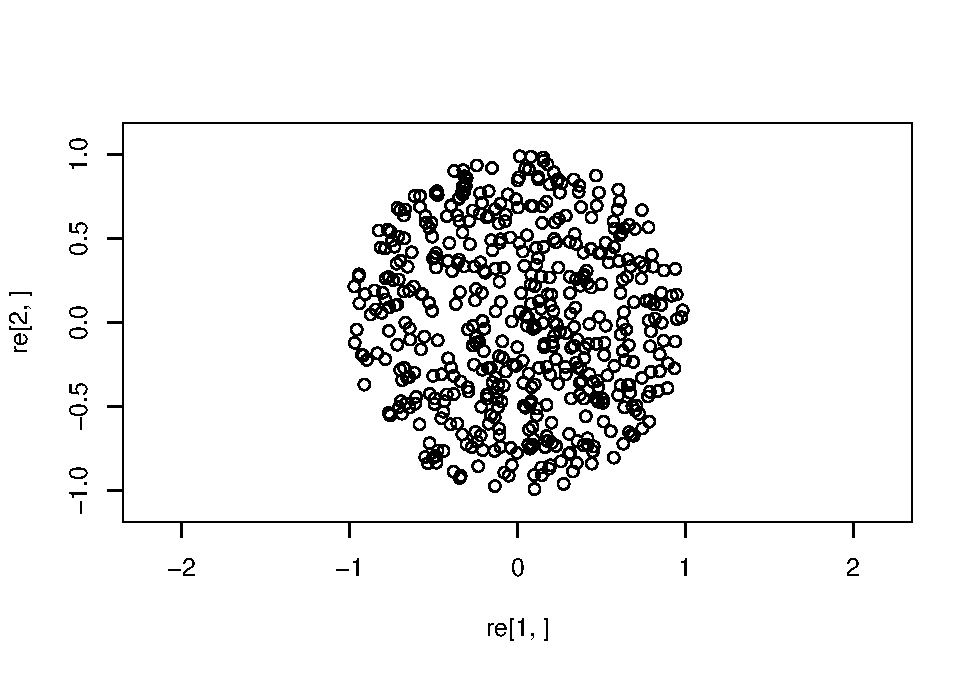
\includegraphics{randomTP_files/figure-latex/unnamed-chunk-3-1.pdf}

\hypertarget{acceptencerejection-sampling-from-a-pdf}{%
\subsection{Acceptence/Rejection: Sampling from a pdf}\label{acceptencerejection-sampling-from-a-pdf}}

The acceptance/rejection method can used to sample from a pdf.

\begin{itemize}
\item
  Suppose we want to generate a random variable \(X\) with pdf \(f\).
\item
  Suppose \(f\) is a complicated pdf with an inverse that is difficult to compute.
\item
  Suppose we can easily generate \(Y\) which has pdf \(g\).
\item
  Suppose there exists \(M\) so that \(f(x) \leq M g(x)\).
\item
  Then you are in good shape!
\end{itemize}

\hypertarget{procedure}{%
\subsection{Procedure}\label{procedure}}

\begin{itemize}
\tightlist
\item
  Let \(U\) be uniformly distirbuted on \([0,1]\) and independent of \(Y\)
\item
  Sample from \((U, Y) = (u, y)\)
\item
  Check if
  \[ u \leq  \frac{f(y)}{M \cdot g(y)}\]
\item
  If the inequality holds, accept the value of \(y\), and report \(X=y\); reject otherwise, and repeat.
\end{itemize}

\hypertarget{proof-of-method}{%
\subsection{Proof of method}\label{proof-of-method}}

\begin{proof}
\iffalse{} {Proof. } \fi{}Observe that by the change of variables formula and Fubini, we have
\begin{eqnarray*}
 \mathbb{P}(Y \leq x, MU g(Y) \leq f(Y)) 
&=& \int_{-\infty} ^x \int_0 ^1 \mathbf{1}[Mu g(y) \leq f(y)]g(y)dudy \\
&=&  \int_{-\infty} ^x  \mathbb{P}[U \leq f(y)/Mg(y)] \cdot g(y) dy \\
&=&  \int_{-\infty} ^x f(y)/M dy \\
&=&  F(x)/M.
\end{eqnarray*}

Thus

\[
\mathbb{P}(Y \leq x | MU g(Y) \leq f(Y)) = F(x).
\]
So, given that we accepted the distribution of \(Y\), is the distribution of \(X\), that random variable we want to sample/simulate.
\end{proof}

\hypertarget{a-simple-example-with-code}{%
\subsection{A simple example with code}\label{a-simple-example-with-code}}

\begin{itemize}
\tightlist
\item
  Consider the pdf \(f(x) = 3x^2\) on the unit interval \([0,1]\).
\item
  Consider the pdf \(g(x) = 1\) on the unit interval.
\item
  Of course, \(f(x) \leq 3 g(x)\).
\end{itemize}

\begin{Shaded}
\begin{Highlighting}[]
\NormalTok{samplef }\OtherTok{\textless{}{-}} \ControlFlowTok{function}\NormalTok{()\{}
\NormalTok{x}\OtherTok{=}\SpecialCharTok{{-}}\DecValTok{1}
\ControlFlowTok{while}\NormalTok{(x}\SpecialCharTok{=={-}}\DecValTok{1}\NormalTok{)\{}
\NormalTok{y }\OtherTok{=} \FunctionTok{runif}\NormalTok{(}\DecValTok{1}\NormalTok{)}
\NormalTok{u }\OtherTok{=} \FunctionTok{runif}\NormalTok{(}\DecValTok{1}\NormalTok{)}
\ControlFlowTok{if}\NormalTok{( u}\SpecialCharTok{*}\DecValTok{3} \SpecialCharTok{\textless{}} \DecValTok{3}\SpecialCharTok{*}\NormalTok{(y}\SpecialCharTok{\^{}}\DecValTok{2}\NormalTok{))\{ x}\OtherTok{\textless{}{-}}\NormalTok{ y\}}
\NormalTok{\}}
\NormalTok{x}
\NormalTok{\}}
\end{Highlighting}
\end{Shaded}

\begin{Shaded}
\begin{Highlighting}[]
\NormalTok{accepted}\OtherTok{=}\FunctionTok{replicate}\NormalTok{(}\DecValTok{100000}\NormalTok{, }\FunctionTok{samplef}\NormalTok{())}
\NormalTok{B }\OtherTok{=} \FunctionTok{seq}\NormalTok{(}\DecValTok{0}\NormalTok{, }\DecValTok{1}\NormalTok{, }\AttributeTok{by=}\FloatTok{0.01}\NormalTok{)}
\FunctionTok{hist}\NormalTok{(accepted, }\AttributeTok{prob=}\ConstantTok{TRUE}\NormalTok{, B)}
\end{Highlighting}
\end{Shaded}

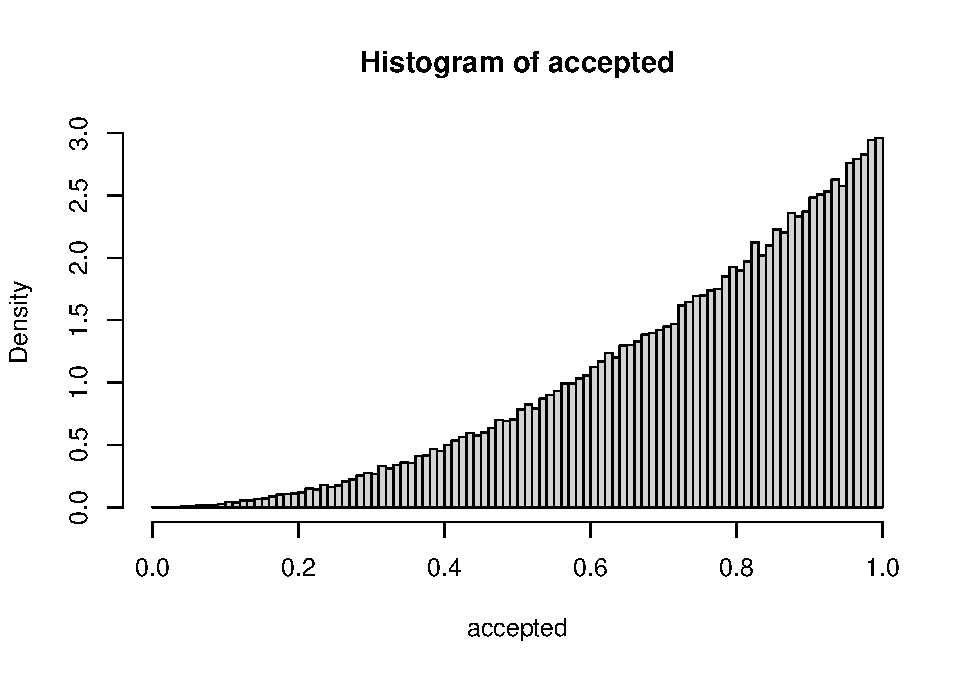
\includegraphics{randomTP_files/figure-latex/unnamed-chunk-6-1.pdf}

\hypertarget{summary}{%
\section{Summary}\label{summary}}

\begin{itemize}
\tightlist
\item
  We rediscovered probability spaces
\item
  The central role of uniform random variables in theory and practice
\item
  Sampling methods such as acceptance/rejection
\end{itemize}

\hypertarget{version-27-april-2021}{%
\section{Version: 27 April 2021}\label{version-27-april-2021}}

\begin{itemize}
\tightlist
\item
  \href{https://tsoo-math.github.io/ucl/randomTP.Rmd}{Rmd Source}
\end{itemize}

\end{document}
